\chapter{Développement de la contrainte de régularité temporelle pour $\beta = 0$ et $\beta = 2$}\label{annex:smoothNMF}

Inspiré par l'article \cite{essid2013smooth} et \cite{fevotte_algorithms_2011}, les algorithmes de mise à jour de la NMF avec une contrainte de régularité temporelle sont développés. initialement développé pour la divergence K-L, elle est étendue au cas de la distance EUC et de la divergence I-S. Les détails des calculs menant aux algorithmes sont présentés ici. Ils n'ont pas été implémentés et utilisés dans le cadre des travaux de la thèse.

\section{Cas de la distance Euclidienne}
On pose le calcul de la fonction de coût pour la NMF avec une distance EUC et la contrainte :

\begin{align}
C(\mathbf{H}) &= D_2(\mathbf{V} \Vert \mathbf{WH}) + \alpha_t C_{MM}(\mathbf{H})\\
 &= \frac{1}{2}\sum_n(\mathbf{v}_n-\mathbf{Wh}_n)^2+\alpha\lambda L(\mathbf{h}_{n}; \mathbf{h}_{(n+1)}, \mathbf{h}_{(n-1)}) 
\end{align}
avec $\lambda = \Vert w \Vert$, la terme de normalisation des matrices $\mathbf{W}$ et $\alpha$ la pondération de la contrainte. On définit $\mathbf{h}$, la valeur de $\mathbf{h}$ à déterminer à l'itération $i+1$, $\mathbf{\tilde{h}}$, sa valeur à l'itération $i$ et $\mathbf{\tilde{v}}_f = \left[\mathbf{W}\tilde{\textbf{h}}\right]$.
En suivant la méthode de \textit{majorisation-minimisation}, une fonction auxiliaire $G_{SM}(\mathbf{h}_{k}\vert \mathbf{\tilde{h}}_{k})$ est définie : 

\begin{equation}
G_{SM}(\mathbf{h}_{n}\vert \mathbf{\tilde{h}}_{n}) = G_{2}(\mathbf{h}_{n}\vert \mathbf{\tilde{h}}_{n})+\alpha_t L(\mathbf{h}_{n}; \mathbf{h}_{(n+1)}, \mathbf{h}_{(n-1)})
\end{equation}


\begin{align}
G_{2}(\mathbf{h}_{n}\vert \mathbf{\tilde{h}}_{n}) &= \frac{1}{2}\sum_{f} \sum_k \frac{w_{fk} \tilde{h}_{kn} v_{fn}^2}{\tilde{v}_{fn}}-2 w_{fk} h_{kn} v_{fn}+w_{fk}\frac{h_{k}^2}{\tilde{h}_{k}}\tilde{v}_{fn}
\\
L(\mathbf{h}_{n}; \mathbf{h}_{(n+1)}, \mathbf{h}_{(n-1)}) &= \frac{1}{2}\sum_{k}\lambda_k^2 \left[ \left(h_{k(n+1)}-h_{kn}\right)^2+\left(h_{kn}-h_{k(n-1)}\right)^2 \right]\\
&= \sum_k \lambda_k^2 \left[ h_{kn}^2- h_{kn}\left(h_{k(n+1)}+h_{k(n-1)}\right)+\frac{1}{2} \left(h_{k(n+1)}^2+h_{k(n-1)}^2\right) \right].
\end{align}
 
La minimisation de la fonction $G_{SM}(\mathbf{h}_{n}\vert \mathbf{\tilde{h}}_{n})$ est alors déterminée en trouvant les zéros de son gradient $\nabla_{h_k} G_{SM}(\mathbf{h}_{n}\vert \mathbf{\tilde{h}}_{n})$ :

\begin{align}
\nabla_{h_{k}} G_{SM}(\mathbf{h}_{n}\vert \mathbf{\tilde{h}}_{n}) &= \nabla_{h_{k}} G_{2}(\mathbf{h}_{n}\vert \mathbf{\tilde{h}}_{n}) + \alpha_t \nabla_{h_{k}} L(\mathbf{h}_{n}; \mathbf{h}_{(n+1)}, \mathbf{h}_{(n-1)})\\
\begin{split}
    ={}& \sum_{f} \sum_{k} \left( 2\alpha_t \lambda_k^2 + \frac{w_{fk} v_{fn}}{\tilde{h}_{kn}}\right)h_{kn} \\
    & - \left(w_{fk} v_{fn} + \alpha_t \lambda_k^2 \left(h_{k(n+1)}+h_{k(n-1)}\right)\right) 
    \end{split}\\
\begin{split}
    ={}& \frac{1}{2}\sum_{f} \sum_{k} -2 w_{fk} v_{fn} + 2 w_{fk} v_{fn} \frac{h_{kn}}{\tilde{h}_{kn}} \\
    & + \alpha_t \lambda_k^2 \left( 2 h_{kn}- (h_{k(n+1)}+h_{k(n-1)}) \right)\label{eq:smooth_2}
\end{split}
\end{align}


L'équation \ref{eq:smooth_2} est alors résolue et permet d'obtenir l'expression des mises à jour de $h_{kn}$ : 

\begin{equation}\label{eq:smooth_beta2}
\fbox{$
h_{kn} = \frac{w_{fk} v_{fn}+\alpha_t  \lambda_k^2 \left(\tilde{h}_{k(n+1)}+\tilde{h}_{k(n-1)})\right)}{2\alpha_t \lambda_k^2 + \cfrac{w_{fk} v_{fn}} {\tilde{h}_{kn}}}$}
\end{equation}
pour $n \in \lbrace 2, N-1 \rbrace$. Dans le cas où $\alpha_t$ = 0, on retrouve bien l' algorithme \ref{eq:update_hk}. Pour $n = 1$, on obtient ; 

\begin{equation}
h_{k1} = \frac{w_{fk} v_{f1}+\alpha_t \lambda_k^2 \tilde{h}_{k2})}{2\alpha_t \lambda_k^2 + \cfrac{w_{fk} v_{f1}}{\tilde{h}_{k1}}}.
\end{equation}

Et pour $n = N$, l'équation \ref{eq:smooth_beta2} devient 
\begin{equation}
h_{kN} = \frac{w_{fk} v_{fN}+\alpha_t  \lambda_k^2 \tilde{h}_{kN}}{2\alpha_t \lambda_k^2 + \cfrac{w_{fk} v_{fN}} {\tilde{h}_{kN}}}.
\end{equation}

Pour illustrer l'impact de la pondération, une scène de 30 secondes est générée comprenant un passage de voiture suivi de sifflements d'oiseaux. Le dictionnaire $\mathbf{W}$ est composé de 5 éléments \textit{trafic} et 5 éléments \textit{oiseaux} construit à partir de 5 échantillons pour chaque classe de son et avec $w_t = all$. La NMF supervisée est appliquée sur cette scène afin d'en déduire le niveau sonore du trafic. On illustre en Figure \ref{fig:smooth_2} l'impact de cette contrainte pour $\alpha_t = \lbrace 0,~2\rbrace$. 

\begin{figure}[h]
\centering
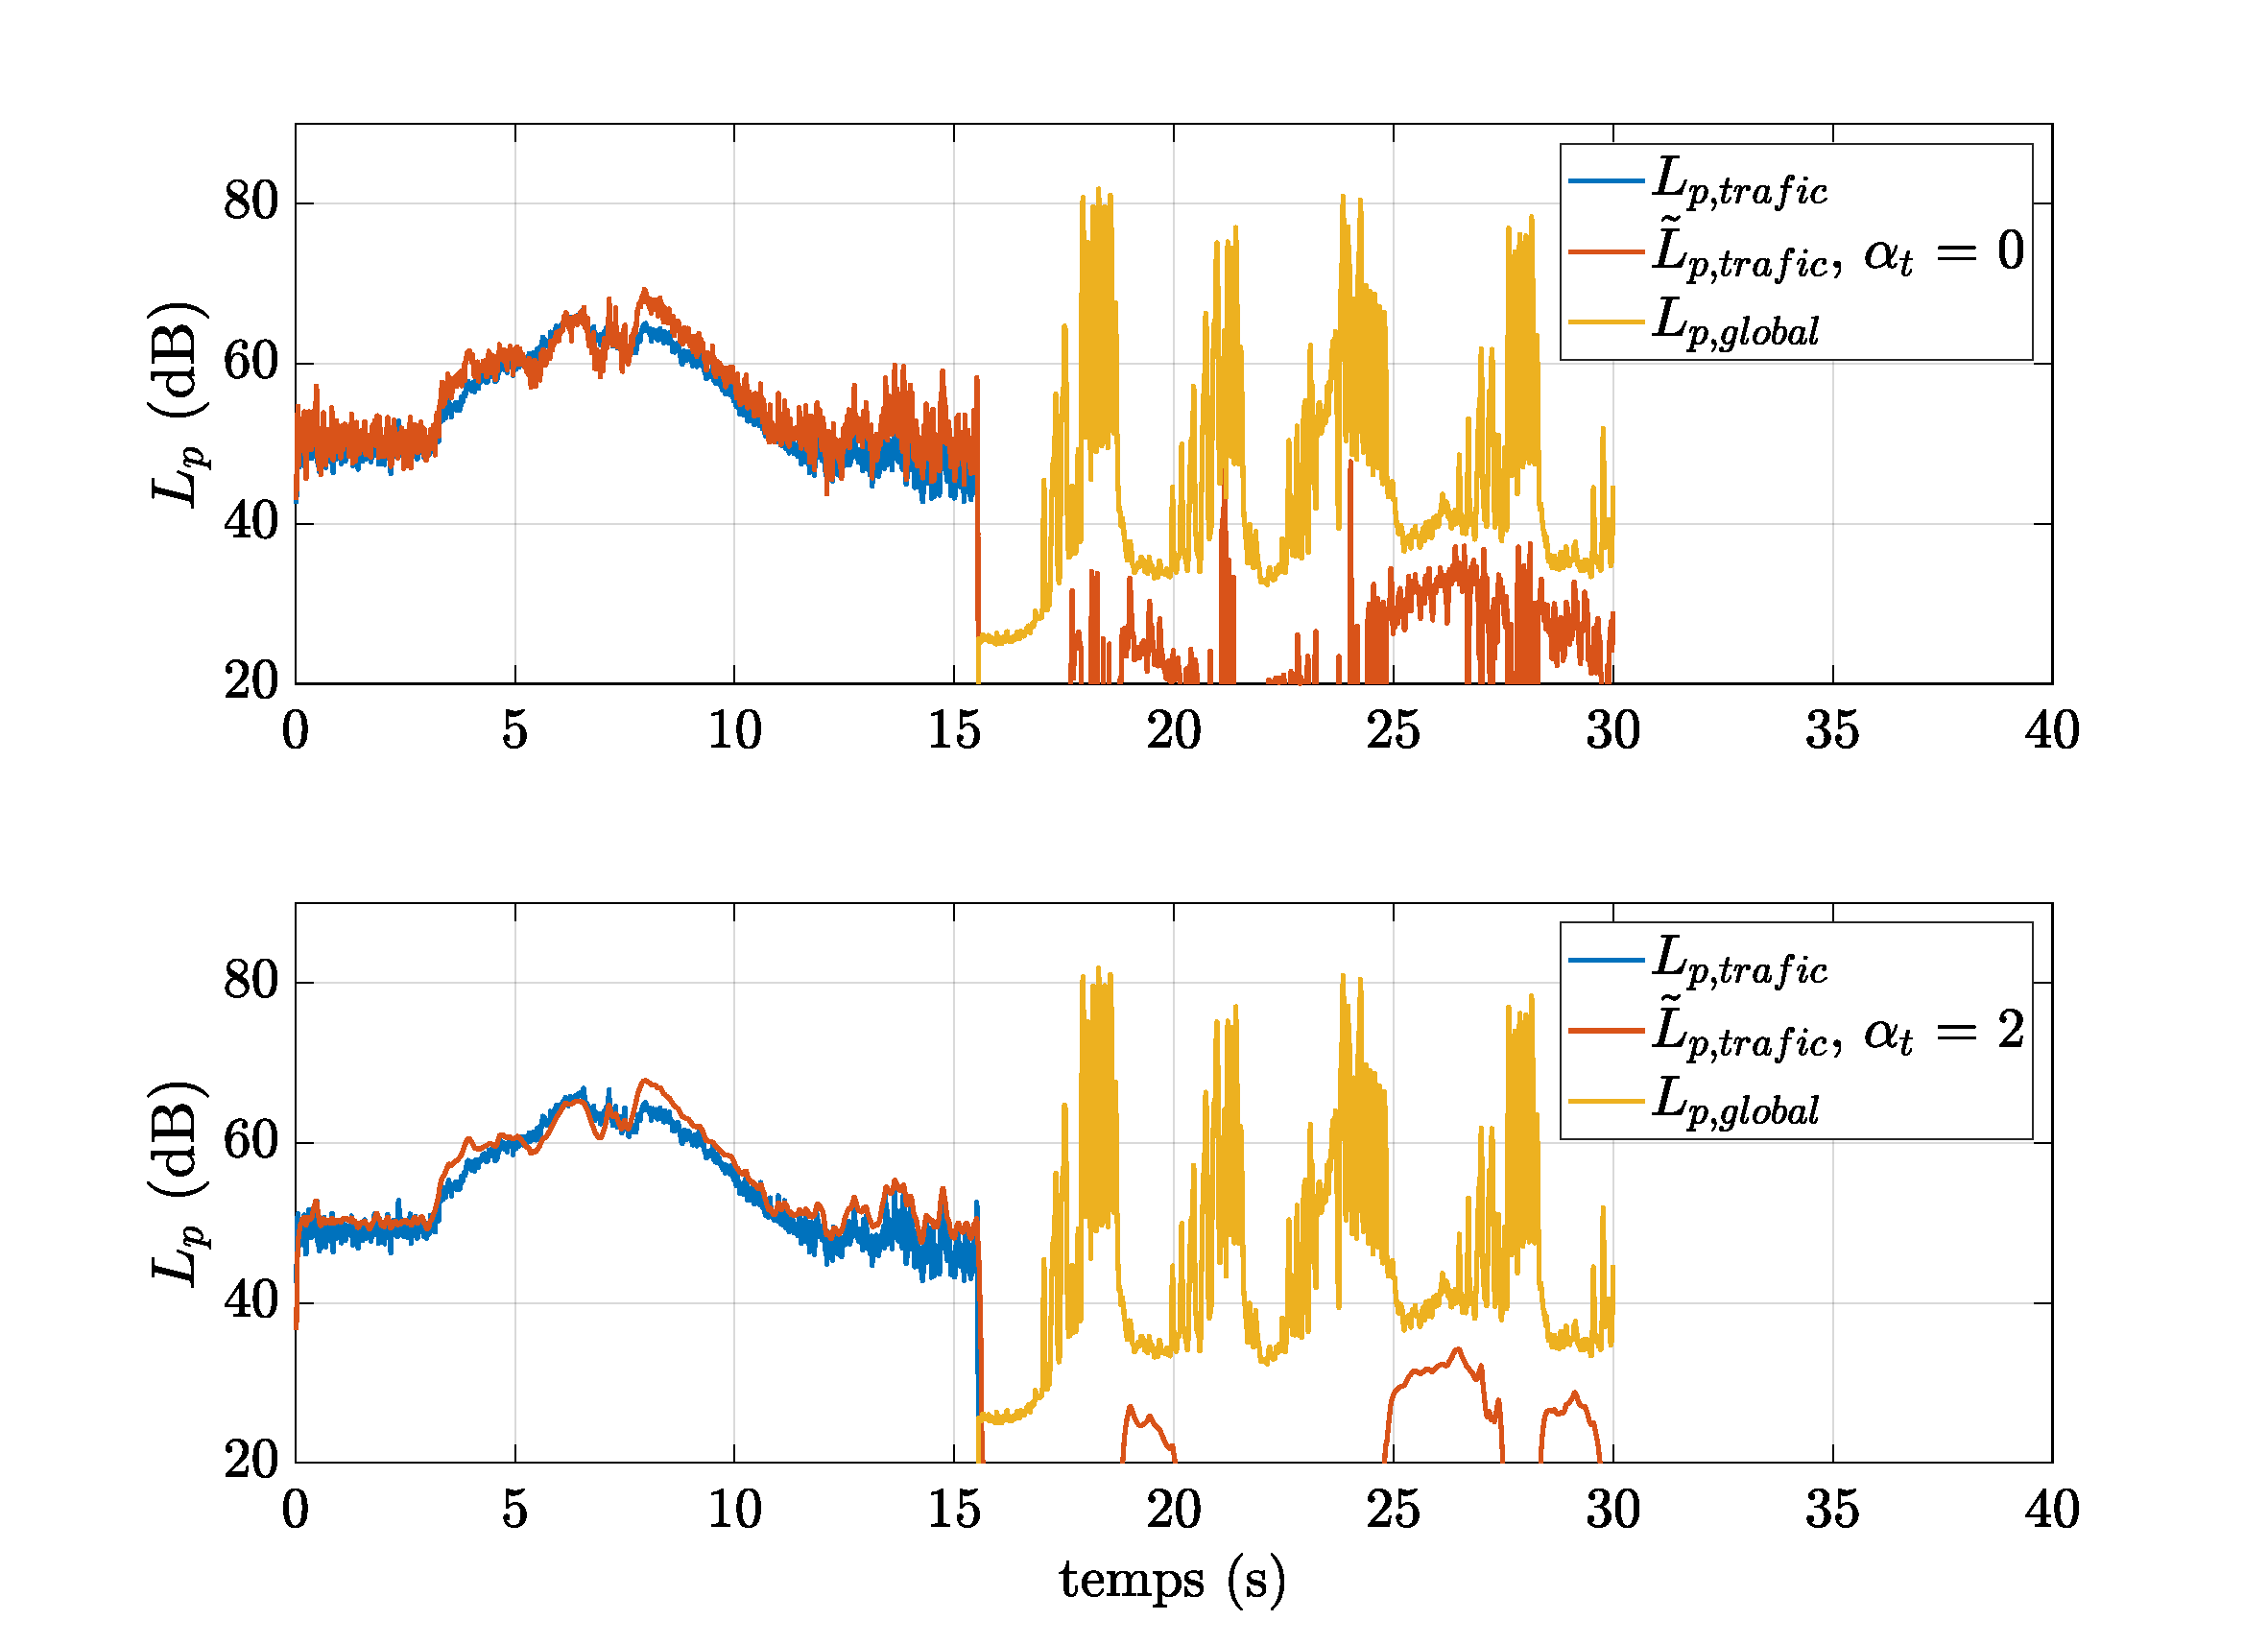
\includegraphics[width=.9\linewidth]{./figures/NMF/LpSmooth_2.pdf}
\caption{Influence de la contrainte de régularité temporelle pour $\beta$ = 2 selon l'algorithme obtenu par \textit{majorisation-minimisation}.}
\label{fig:smooth_2}
\end{figure}


\section{Cas de la divergence d'Itakura-Saïto}
Dans le cas d'une divergence I-S, le problème est similaire avec

\begin{align}
C(\mathbf{H}) &= D_0(\mathbf{V} \Vert \mathbf{WH}) + \alpha_t C_{MM}(\mathbf{H})\\
 &= \sum_k\frac{\mathbf{v}_n}{\mathbf{Wh}_n}-\log \frac{\mathbf{v}_n}{\mathbf{Wh}_n}-1+\alpha_t L(\mathbf{h}_{n}; \mathbf{h}_{(n+1)}, \mathbf{h}_{(n-1)}) 
\end{align}

La fonction auxiliaire $G_0(\mathbf{h}_{n}\vert \mathbf{\tilde{h}}_{n})$ n'est toutefois pas la même : 

\begin{equation}
G_0(\mathbf{h}_n\vert \mathbf{\tilde{h}}_n) = \sum_f \sum_k \left[  \frac{w_{fk} \tilde{h}_{kn}}{\tilde{v}_{fn}}v_{fn} \frac{\tilde{h}_{kn}}{\tilde{v}_{fn} h_{kn}} + \log \tilde{v}_{fn}+ \frac{1}{\tilde{v}_{fn}}(w_{fk}(h_{kn}-\tilde{h}_{kn}) + v_f(\log v_{fn} - 1)\right]
\end{equation}

\begin{align}
\nabla_{h_{k}} G_{SM}(\mathbf{h}_n\vert \mathbf{\tilde{h}}_n) &= \nabla_{h_{k}} G_0(\mathbf{h}_n\vert \mathbf{\tilde{h}}_n) + \alpha_t \nabla_{h_{k}} L(\mathbf{h}_{n}; \mathbf{h}_{(n+1)}, \mathbf{h}_{(n-1)})\\
\begin{split}
=&{} \sum_f \sum_k -w_{fk}\frac{\tilde{h}_{kn}^2}{h_{kn}^2} \frac{v_{fn}}{\tilde{v}_{fn}^2}+\frac{w_{fk}}{\tilde{v}_{fn}}\\
&  + \alpha_t \lambda_k^2 \left[ 2 h_{kn} - \left(h_{k(n+1)}+h_{k(n-1)}\right) \right]
\end{split}\\
\begin{split}
 =&{} \alpha_t\lambda^2 \sum_f \sum_k 2h_{kn}^3+\left[\frac{w_{fk}}{\tilde{v}_{fn}} - \alpha_t \lambda_k^2\left( h_{k(n+1)}+h_{k(n-1)}\right) \right]h_{kn}^2\\
 & - w_{fk}\frac{v_{fn}}{\tilde{v}_{fn}^2}\tilde{h}_{kn}^2 
 \end{split}\label{eq:eq_mimiser_smooth}
\end{align}

On obtient un problème de type équation du 3\ieme{} ordre : $ax^3+bx^2+cx+d = 0$ avec 
\begin{itemize}
\item $a = 2\alpha_t\lambda^2$, 
\item $b = \frac{w_{fk}}{\tilde{v}_f} - \alpha_t \lambda_k^2\left(h_{k(n+1)}+h_{k(n-1)}\right)$, 
\item $c = 0$, 
\item $d = -w_{fk}\frac{v_{fn}}{\tilde{v}_{fn}}\tilde{h}_{kn}^2$.
\end{itemize}

Cette polynôme d'ordre 3 se résout à l'aide de la méthode de Cardan \cite{nickalls1993new}, qui dans le cas présent, s'exprime sous la forme : 

\begin{equation}
x^3+\frac{b}{a}x^2+\frac{d}{a} = 0.
\end{equation}

Dans un premier temps, un premier changement de variable est effectué $x = X - \frac{b}{3a}$ et on obtient : 

\begin{equation}\label{eq:cardan}
X^3+pX+q = 0
\end{equation}

avec $p = -\frac{b^2}{3a^2}$ et $q = \frac{2b^3}{27a^3}+\frac{d}{a}$. La variable $X$ est alors décomposée en deux variables complexes : $X = u+v$. L'équation \ref{eq:cardan} devient alors : 

\begin{equation}\label{eq:u_v}
u^3+v^3+(3uv+p)(u+v)+q = 0.
\end{equation}

L'équation \ref{eq:u_v}, pour être résolue, implique alors deux conditions  : 
\begin{subequations}\label{eq:condition1}
\begin{align}
3uv &= -p,\\
u^3+v^3 &= -q.
\end{align}
\end{subequations}

Du système d'équations \ref{eq:condition1}, on obtient  : 

\begin{subequations}\label{eq:condition2}
\begin{align}
u^3+v^3 &= -q,\\
u^3v^3 &= -\frac{p^3}{27}.
\end{align}
\end{subequations}

Si on réalise un nouveau changement de variable $u^3 = U$ et $v^3 = V$, on exprime le système d'équation \ref{eq:condition2} comme des polynômes de second degré : 

\begin{subequations}\label{eq:polyUV}
\begin{align}
U^2+qU-\frac{p^3}{27} &= 0,\\
V^2+qV-\frac{p^3}{27} &= 0.
\end{align}
\end{subequations}

Le système \ref{eq:polyUV} se résout classiquement : 

\begin{equation}
\Delta_U = \Delta_V = \Delta = q^2-4\frac{p^3}{27}.
\end{equation}

Les équations \ref{eq:polyUV} ont alors les deux mêmes solutions. Les valeurs de $X$ et solutions de l'équation \ref{eq:cardan} dépendent alors du signe de $\Delta$ : 

\begin{itemize}
\item pour $\Delta >0$, 

\begin{subequations}
\begin{align}
X_1 &= \sqrt[3]{\frac{-q+\sqrt{\Delta}}{2}}+\sqrt[3]{\frac{-q-\sqrt{\Delta}}{2}},\\
X_2 &= j\sqrt[3]{\frac{-q+\sqrt{\Delta}}{2}}+j^2\sqrt[3]{\frac{-q-\sqrt{\Delta}}{2}},\\
X_3 &= j^2\sqrt[3]{\frac{-q+\sqrt{\Delta}}{2}}+j\sqrt[3]{\frac{-q-\sqrt{\Delta}}{2}}
\end{align}
\end{subequations}

avec $j = e^{\sfrac{2i\pi}{3}}$. Une autre forme d'écriture la solution est possible sous une forme trigonométrique : 

\begin{equation}
X_{z} = 2\sqrt{\frac{-p}{3}} \cos \left(\frac{1}{3} \arccos\left(\frac{-q}{2}\sqrt{\frac{27}{-p^3}}\right) + \frac{2(z-1)\pi}{3}\right)
\end{equation}

avec $z \in \left\lbrace 1,2,3 \right\rbrace$.


\item Pour $\Delta = 0$, parmi les 3 solutions possibles, 1 seule solution est réelle : 

\begin{subequations}
\begin{align}
X_1 &= \frac{3q}{p},\\
X_2 &= X_3 = \frac{-3q}{2p}.
\end{align}
\end{subequations}

\item Pour $\Delta < 0$, les équations \ref{eq:polyUV} ont pour solutions 
\begin{align}
S_1 &= \frac{-q+i\sqrt{\vert\Delta \vert}}{2},\\
S_2 &= \frac{-q-i\sqrt{\vert \Delta \vert}}{2}. 
\end{align} 
L'équation \ref{eq:cardan} possède alors une solution réelle et 2 solutions complexes qui sont 
: 

\begin{subequations}
\begin{align}
X_1 &= \sqrt[3]{S_1}+\sqrt[3]{S_2},\\
X_2 &= j\sqrt[3]{S_1}+j^2\sqrt[3]{S_2},\\
X_3 &= j^2\sqrt[3]{S_1}+j\sqrt[3]{S_2}.
\end{align}
\end{subequations}
\end{itemize}

Ainsi, la solution du problème \ref{eq:eq_mimiser_smooth} est donc la valeur $X_z$ qui est réelle et positive parmi les trois solutions possibles et définie selon le signe de $\Delta$ : 

\begin{equation}
\fbox{$
h_{kn} = X_{z}^+-\frac{b}{3a}.
$}
\end{equation}

Le même exemple illustratif que pour $\beta$ = 2 est repris ici en Figure \ref{fig:smooth_0}. On relève que la valeur $\alpha_t$ est bien plus élevée pour la divergence IS ($\alpha_t = 10^7$) que pour la distance EUC en raison de la valeur $d$ et du rapport $\frac{w_{fk}}{\tilde{v}_f}$ de $b$, dans l'équation du 3\ieme{} ordre, qui prennent des valeurs élevés.

\begin{figure}[h]
\centering
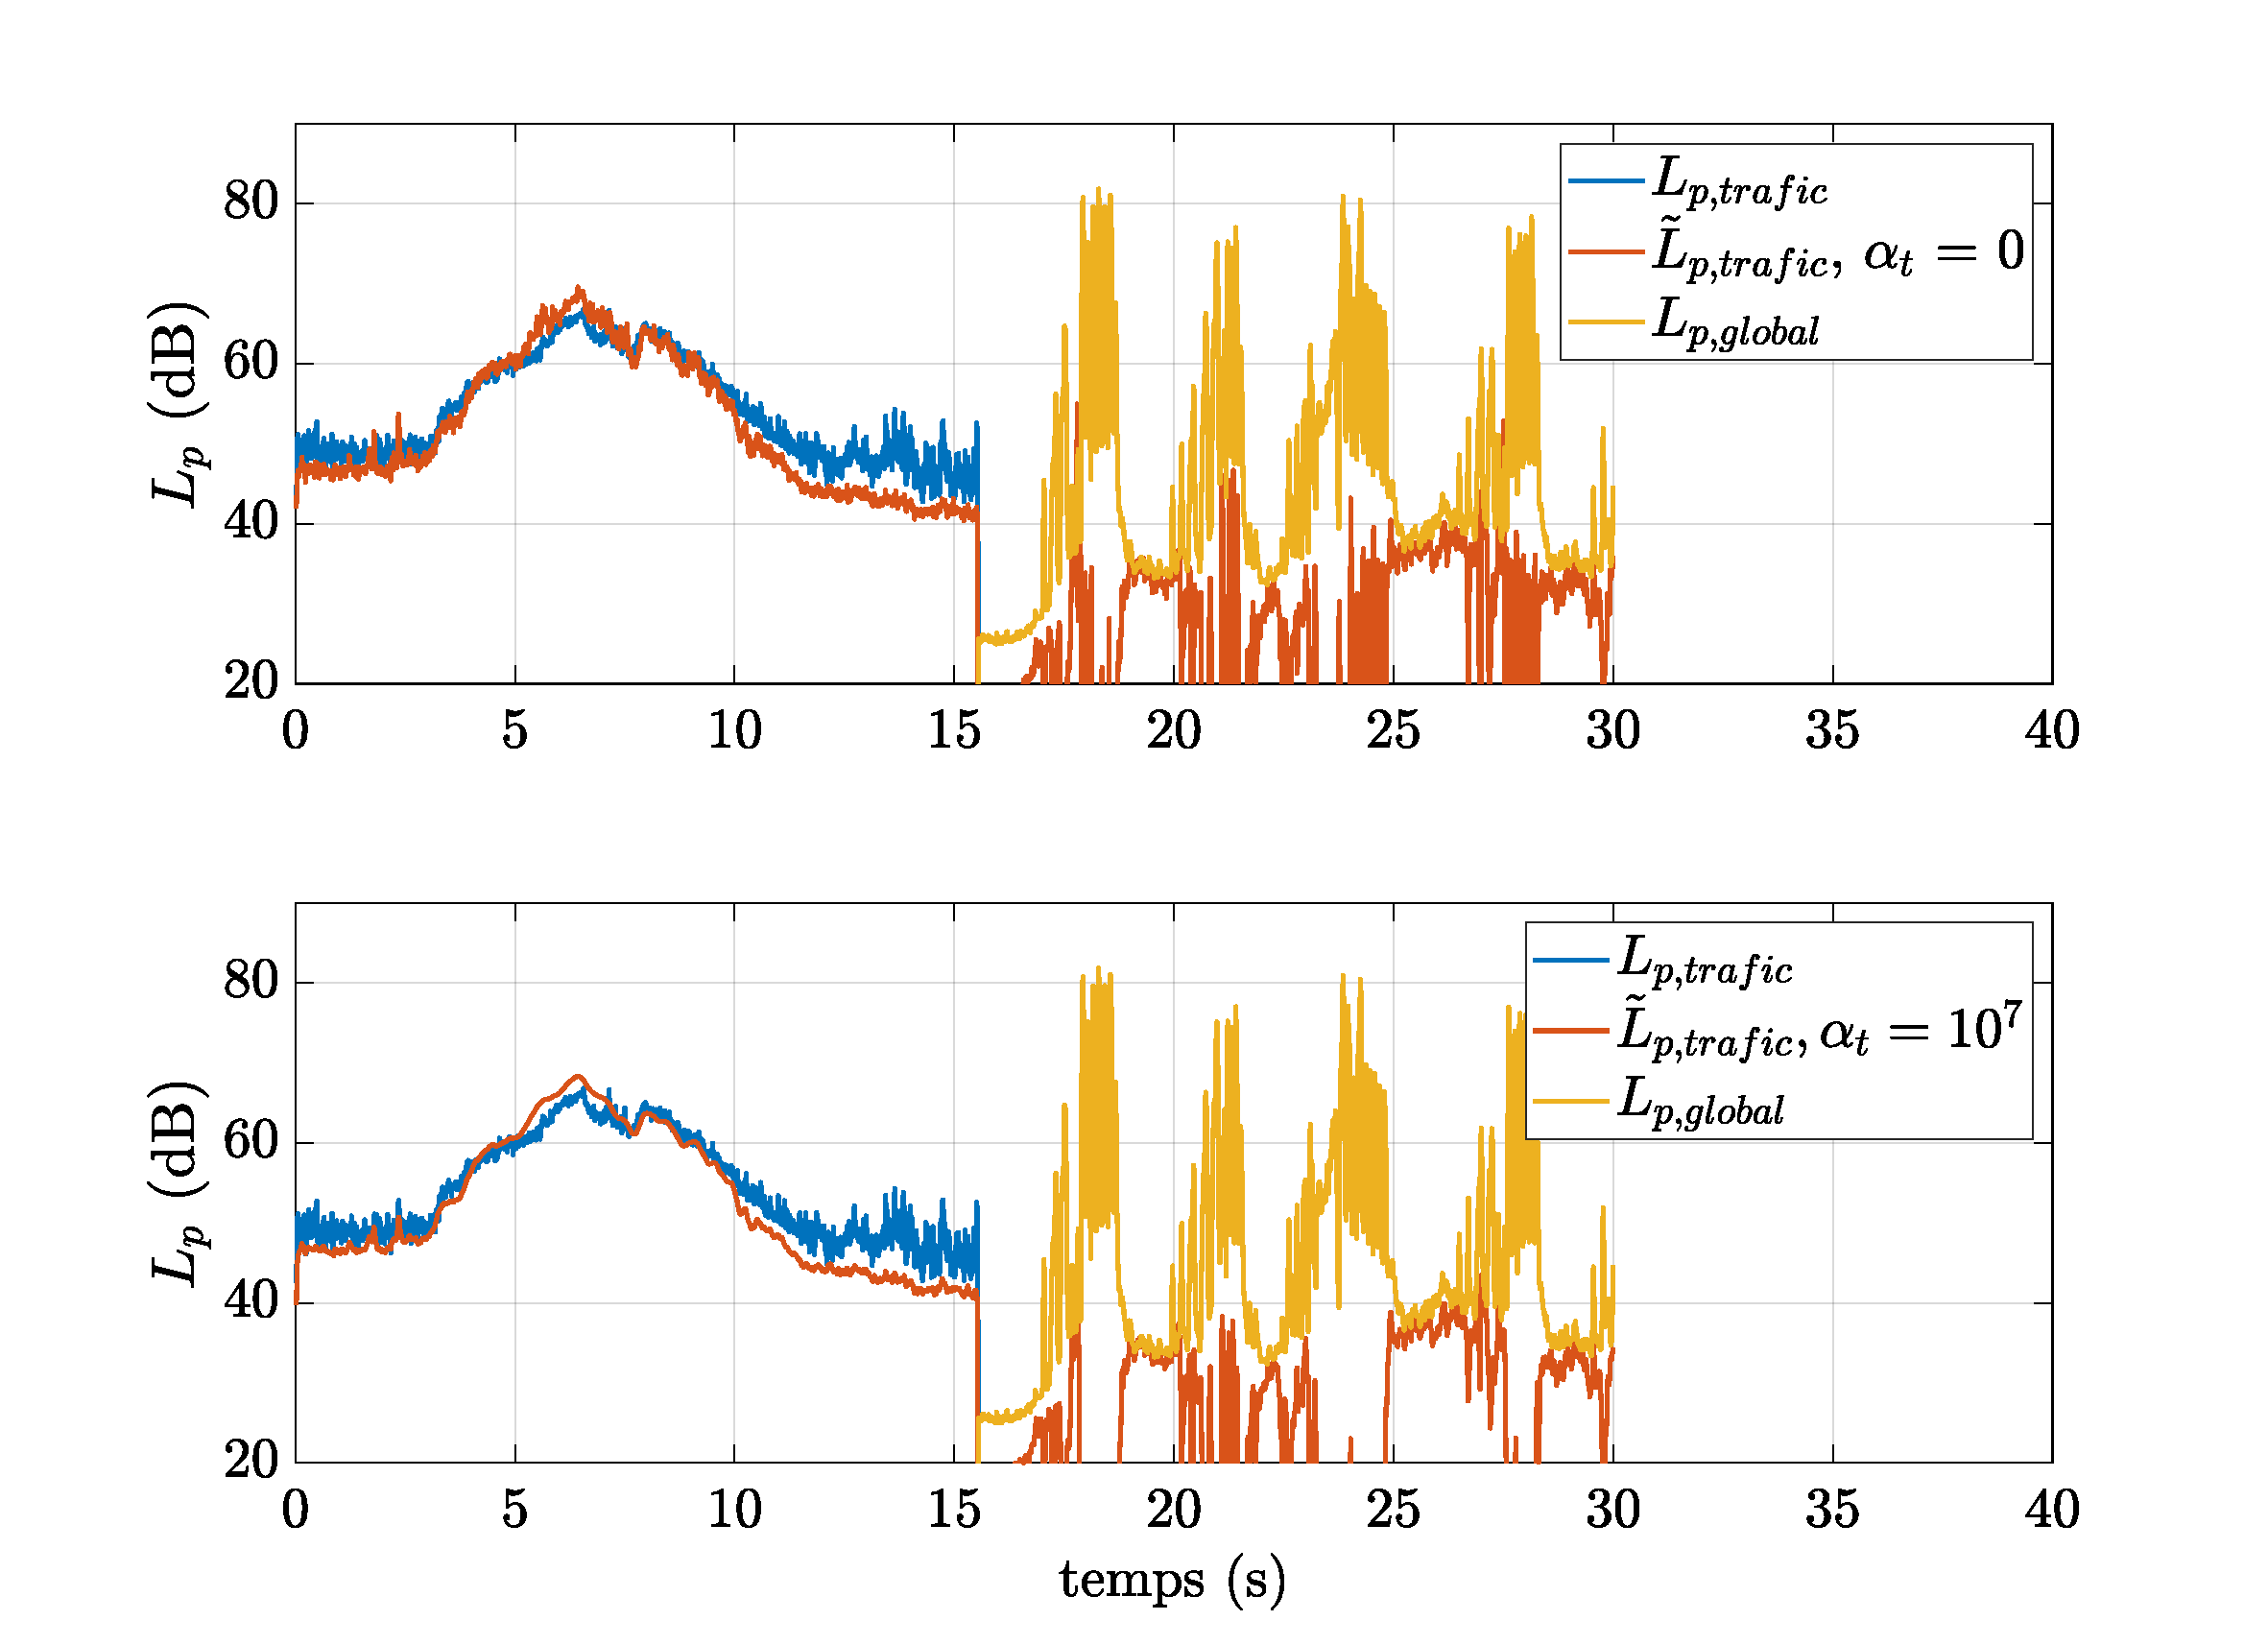
\includegraphics[width=.9\linewidth]{./figures/NMF/LpSmooth_0.pdf}
\caption{Influence de la contrainte de régularité temporelle pour $\beta$ = 0 selon l'algorithme obtenu par \textit{majorisation-minimisation}.}
\label{fig:smooth_0}
\end{figure}
